\documentclass[11pt]{article}
\usepackage{tikz}
\usetikzlibrary{positioning,arrows}
\usepackage[scaled]{helvet}
\renewcommand\familydefault{\sfdefault} 
\usepackage[T1]{fontenc}


\tikzset{
	mynode/.style={draw=none,text centered,text width = 6em},
	myarrow1/.style={->,>=latex,shorten >=1pt,very thick},
	myarrow2/.style={->,>=latex,shorten >=1pt,very thin},
	myarrow3/.style={->,>=latex,shorten >=1pt,thick}
}


\title{}
\author{}


\begin{document}


	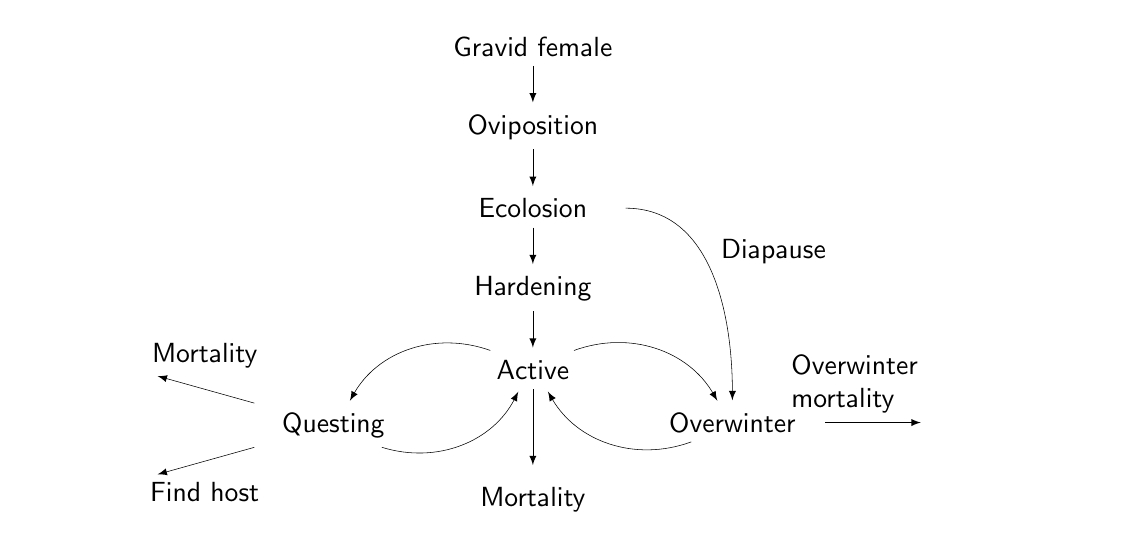
\begin{tikzpicture}[node distance=0.5cm,auto]
		\node[mynode](gravid){Gravid female};
		\node[below = 0.5 cm of gravid,mynode](egg){Oviposition};
		\draw[myarrow2] (gravid) -- (egg);
		\node[below = 0.5 cm of egg,mynode](ecolsion){Ecolosion};
		\draw[myarrow2] (egg) -- (ecolsion);
		\node[below = 0.5 cm of ecolsion,mynode](hardening){Hardening};
		\draw[myarrow2] (ecolsion) -- (hardening);
		\node[below = 0.5 cm of hardening,mynode](active){Active};
		\draw[myarrow2] (hardening) -- (active);
		\node[below right = 0.25 cm of active,mynode](winter){Overwinter};
		\draw[myarrow2] (active) edge[bend left = 40] (winter);
		\draw[myarrow2] (winter) edge[bend left = 40] (active);
		\node[right = 1.25 cm of winter,mynode](dummy1){};
		\draw[myarrow2] (winter) -- (dummy1) node[midway, text width = 6em]{Overwinter mortality};
		\node[below left = 0.25 cm of active,mynode](quest){Questing};
		\draw[myarrow2] (active) edge[bend right = 40] (quest);
		\draw[myarrow2] (quest) edge[bend right = 40] (active);
		\node[above left = 0.5 cm of quest,mynode](dummy2){};
		\draw[myarrow2] (quest) -- (dummy2) node[above = 0.15 cm,midway]{Mortality};
		\node[below left = 0.5 cm of quest,mynode](dummy3){};
		\draw[myarrow2] (quest) -- (dummy3) node[below = 0.15 cm,midway]{Find host};
		\draw[myarrow2, in = 90, out = 0] (ecolsion) to node[midway]{Diapause} (winter);
		\node[below =1cm of active,mynode](dummy3){};
		\draw[myarrow2] (active) -- (dummy3) node[below]{Mortality};

	\end{tikzpicture}
	
\end{document}